% File SDSS2020_SampleExtendedAbstract.tex
\documentclass[10pt]{article}
\usepackage{sdss2020} % Uses Times Roman font (either newtx or times package)
\usepackage{url}
\usepackage{latexsym}
\usepackage{amsmath, amsthm, amsfonts}
\usepackage{algorithm, algorithmic}
\usepackage{graphicx}
\usepackage{adjustbox}
\graphicspath{{images/}}

\title{Artificial Neural Networks and Deep Learning \\
Homework 1}

\author{
  Nicola Dean \\
  10674826 \\
  {\tt nicola.dean \\
  \tt @mail.polimi.it} \\\And
  Marco Fasanella \\
  10617541 \\
  {\tt marco.fasanella \\
  \tt @mail.polimi.it} \\\And
  Raffaello Fornasiere \\
    10790353 \\
    {\tt raffaello.fornasiere \\
    \tt @mail.polimi.it} \\\And
  Christian Spano \\
  10823764 \\
  {\tt christian.spano \\
  \tt @mail.polimi.it} \\}


\date{}

\begin{document}
\maketitle
%\begin{abstract}

%\end{abstract}

%{\bf Keywords:} VGG16, VGG19, Helpful

\section{Introduction}
In order to touch all the important aspects of the procedure of finding the best solution to this classification problem,
we started from our own self-made model to more sophisticated methodologies.\\
 We can summarize our approaches in:
\begin{itemize}
  \item Vanilla network
  \item Transfer Learning and Fine Tuning
  \item Ensemble method
\end{itemize}
Furthermore in all the attempts made, we used two classes, specifically \textbf{created to automate and support the model creation
procedure}:
\begin{itemize}
  \item Dataset Helper
  \item Model Helper
\end{itemize}
Through the continuous attempts, and support of methods in the two helper classes, we managed to find our best model and
reach 0.8691 accuracy in the competition.


\section{Dataset Helper and Model Helper}
In order to ease the development of our best solution, we thought it would have been useful to create two ad-hoc helpers. As a matter of fact, a lot of code is often repeated or many lines of code are needed just to plot or to get insightful results (such as the confusion matrix or the accuracy). In particular, what we did was to create two helpers:
\begin{itemize}
    \item \textbf{Dataset helper}: for dealing with everything related to the dataset; for instance (just for mentioning the most relevant functions) we created functions to perform \textit{augmentation} and \textit{cut-out/cut-mix} of the dataset. Other functions were intended for processing data (e.g., normalization)
    \item \textbf{Model helper}: for dealing with everything related to the models; this helper was intended for easing the construction of models. For instance, we create some functions for plotting insightful graphs (e.g., confusion matrix, residuals, predictions, etc.) and some other functions for managing the models (e.g., save the model in a specified directory or create checkpoints during training)
\end{itemize}
At the end, these helpers indeed turned out to be really helpful. Just with a line we had everything we needed. We firmly think they will turn out to be crucial also in other Deep Learning projects.

\section{First try: vanilla network}
--NICOLA--
-IMG della rete (dal lab) (magari orizzontale)
risultati
considerazioni
\subsection{Batch Normalization}
A first attempt was also adding a Batch Normalization + ReLu Activation Layer before our Pooling layers.\
This lead to poor result due to the fact that the network was too small.

\subsection{Our homemade CNN}
After some attempts on small vanilla networks with poor results we tried to improve the network by adding some more layers with more filters.
We combined different parameters: kernel size, number of filters, number of layers, units of the dense layers.
After some trials we noticed that we were not reaching any significant improvement (very low test scores, around 0.5/0.6 of accuracy).
All of these trials were made with a small dataset (4000 images), but after the work done on augmentation (\ref{subsec:augmentation}) the same model performed much better reaching 0.80/0.85 on test set.
We noticed though the model was not much reliable since on Codalab it performed around 0.78.


\subsection{Augmentation}\label{subsec:augmentation}
Since vanilla networks were not providing good results we decided to focus on data.
First of all we decided to generate a number of images so that the ratio $images_{specie_i}/tot_{images}$ was almost the same for each specie $i=1,\dots,8$.
then we started exploiting all the functionalities of \textbf{ImageDataGenerator} in order to generate as much images as possible so that the network could extract them without overfitting.
By doing this we started reaching higher accuracies deduced that the image dataset should not be smaller then 10k images.
With further search we noticed smaller -- but significant -- improvements until 25k images.
After that we decided to improve the generalization ability of the network by augmenting the images with \textbf{CutMix}, \textbf{MixUp}, \textbf{GridMask} and \textbf{Grayscale}.
This turned out to be another small but significant improvement on the accuracy, reaching 3/4 percentage points on test accuracy, depending also on the model used.



\subsection{Considerations}
Best result consideration and observations \\
Commento da Christian: qui specifichiamo l'importanza della augmentation e che abbiamo pensato potesse risolvere il problema della bassa accuracy (infatti alla fine è megliorato) + che poi abbiamo espanso con cut-out e cut-mix -- magari dire brevemente il perché, secondo noi, con augmentation/cutout è migliorato.
\section{Transfer Learning and Fine Tuning}
We then noticed that we needed a big change on the approach to use, because the homemade
CNN was performant, but not enough. So \textbf{we started using transfer learning and Fine tuning}

\subsection{Approach: Freezing Layers}
The \textit{modus operandi} that will be used from now is: freezing all layers while training on our augmented dataset the keras.application
CNN, and then unlock a small amount of layers to the second phase of training (fine tuning) as near as possible to the output.
\subsection{VGG16}
The first network we decided to utilize with this approach was VGG16. We started from this network mainly because, generally speaking, it has given great results in many different Deep Learning tasks; so, we thought it was a good network to start with. Indeed, at the end, it did not deceive us.\\[0.1cm] More in details, at the very first we trained this network neither applying augmentation nor fine-tuning. By the way, the network architecture was equal to the standard VGG16 one, with 256 neurons in the Dense Layer at the top. However, as expected, we got poor results (an accuracy of about $60\%$). Applying data-augmentation, the accuracy risen up to roughly $70\%$, that is an improvement in accuracy of $10\%$.\\[0.1cm]
At this point, to boost up even more the accuracy, we decided to do fine-tuning treating the number of freezed layer as an hyperparameter to be learned. Indeed, we trained the network with $k$ freezed layers and we pick up the one such that
\begin{equation*}
    k^* = \underset{k}{\operatorname{argmax}}\{test\_accuracy_{k}\}
\end{equation*}
\subsubsection{Results}
The best number of freezed layers turned out to be $k=8$. Setting this parameter to this 'optimal' value, we got a test accuracy of nearly $0.85$, against $0.8325$ on Codalab. This has been our first best result. That's why further tests have been done. For instance, we tried to change the number of neurons, add more Dense Layers, and change some parameters of the augmentation but all these tests failed since they made the test-accuracy dropping down.\\[0.1cm]
The only test that passed successfully -- even though with very little improvement -- was to apply the more advanced augmentation we mentioned in subsection 3.3. As a matter of fact, this improved dramatically the test accuracy boosting it up to roughly 0.94. However, it provided very little improvement on Codalab, i.e., an accuracy of 0.8381. No other best results have been received with this network and since we were stuck with these results, we thought it was reasonable to explore other pre-trained networks.
\subsection{VGG19}
VGG-19 is a convolutional neural network that is 19 layers deep, so we kept the freezed layers in the range of the first 8-14.\\
Different Data Augmentations (with different seeds and augmentation parameters) were performed between the two phases,
to even increase randomisation in the two training processes.
\subsubsection{Results}
\begin{table}[ht]
\centering
\begin{adjustbox}{width=240}
\small
\begin{tabular}{|c|l|l|l|l|l}

\hline \bf Freezed Layers & \bf Accuracy & \bf Precision & \bf Recall & \bf F1 \\ \hline
8 & 0.8169 & 0.7989 & 0.7651 & 0.763\\
9 & 0.8225 & 0.8181 & 0.7682 & 0.7776\\
10 & 0.8338 & 0.8161 & 0.7929 & 0.8001\\
11 & 0.7577 & 0.7109 & 0.715 & 0.7048\\
12 & 0.7944 & 0.766 & 0.7504 & 0.7489\\
13 & 0.8028 & 0.7806 & 0.754 & 0.7596\\
\hline
\end{tabular}
\end{adjustbox}
\caption{Results with Transfer Learning and Number of freezed layers for VGG19.}
\end{table}


\begin{figure}[ht]
\begin{center}
\centerline{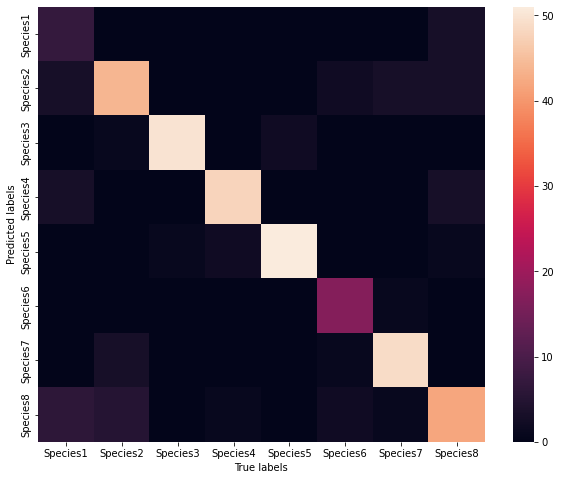
\includegraphics[width=\columnwidth]{VGG19_best}}
\caption{Confusion Matrix of best configuration with VGG19.}
\label{bayespic}
\end{center}
\end{figure}
\subsubsection{Considerations}
One of the most particular observation that we can made after experimenting the first attempts of freezing, is that freezing the net
until the pooling and not between convolutions leads to a better accuracy.

\subsubsection{Results}
\subsection{Xception}
Xception is the evolution google proposed to their \textbf{"Inception-v3"} model, this model contain \textbf{131 layers} of \textbf{"depthwise separable convolution"}.\\
We decided to try this model to see if this particular kind of convolution would extract better features for our model and if this would increase Specie1 and Specie6 F1.\\
The best result was given, surprisingly, by unlocking the full network and using a dense of 256 with global avg pooling but
unfortunatly the performance obtained wasnt so different from our best model at the time, VGG16.

\begin{table}[ht]
  \centering
  \begin{adjustbox}{width=240}
  \small
  \begin{tabular}{|c|l|l|l|l|l}
  
  \hline \bf Freezed Layers & \bf Accuracy & \bf Precision & \bf Recall & \bf F1 \\ \hline
  Transfer-Learn & 0.5734 & 0.5942 & 0.5344 & 0.5376\\
  20 & 0.6328 & 0.5903 & 0.5855 & 0.5852\\
  15 &  &  &  & \\
  1 & 0.8136 & 0.7869 & 0.7751 & 0.7763\\
  \hline
  \end{tabular}
  \end{adjustbox}
  \caption{Some of the best results of FineTuning using Xception. The one with 15-freezed layers has been lost. However, similar results of 20-freezed layers have been obtained (around 0.6 for all the metrics).}
  \end{table}
\subsection{Other Models}
In parallel to fine tuning we had tried different modify to the "home made CNN", one of them was adding skip layers to it to avoid \textbf{vanishing gradient}.\\
We failed to implement them in a performant way, but this bring us to the next model of this FineTuning section: Resnet50-v2.\\
We thought that maybe we were doing something wrong with skip layer, so to prove it we decided to give a try to Resnet.
\subsubsection{Resnet}
Unfortunatly during the various modify of the notebook we lost the cell with the saved "old performaces" and we have only the ones of the best model we get out of Resnet.\\
We had different try on the Final Dense size and the best we could get on base model was with Flattening + Dense of 256 + Dropout 0.2
With 
\subsubsection{GoogleNet}
Just to have a broad exploration and not leaving any doubt on which could be the most power pre-trained network, we decided to give a chance to GoogLeNet. At first, just for clarity, we did not analyse this network in deep and the reasons are here explained.\\[0.1cm]
As usual, we trained the standard GoogLeNet architecture but we noticed immediately a bad behaviour: just after a bunch of epochs the model started to overfit. Besides this point, the accuracy on the validation test fluctuated abruptly passing, for instance, from 0.40 to 0.80 at each epoch. This make us a little distrustful of this network, also because we already found other more promising networks. Thus, we abandoned any further tests on this network.
\subsection{EfficientNet}
As last option we decided to give a try to one of the "BIG" models on keras.application;
Initialy we were discoraged by the huge number of parameter (on colab we hadn't managed to load it due to ram issue for example)
but we wanted to give it a try since it's architecture was different from already tried models, and on keras.application was the best on TOP1 accuracy.\\
As already said, it was a little hard to work with this model given our resources so we used an approach not 100\% correct.
Thats said, to select the best hyperparameter we started to train only few epochs and keep running ONLY if it was promising (probably not the best approach).\\
The model resulted to be promising, since the simple transfer learning managed to get 71\% of accuracy localy, and then we started experimenting fine tuning.\\
We discovered that with a big number of freezed layers during fine tuning thare was no significant improvements.\\
Those improvements come when the num of freezed layers was around 200, 100, precisely this last one was the best with an 85/86\% 
After this, since both Resnet50 and Xception was performing well with "FULL unfreezed" we tried, for curiosity, to apply 30 more epochs with full unfreezed layers and discovered this give the model good increase on performances , precisely of 2/3 \% localy!!!
We tried also the opposite (first full unfreezed and then 100 layer) but this was not effective,actualy it performed worst.


\section{Ensemble}
The ensemble techniques consist into combining multiple models together to create a more robust and accurate one.\\
The idea behind is that we can take our best models, and apply a majority voting on the predicted species.
This will grant more robustness, since wrong choice come from majority of models predicting wrong species.

The improvement was as expected, pretty high, but localy we get a "biased" result since the EfficientNet was trained using a different random seed so different test/train split.. and was too late to retrain such a huge model.
so we will use CodaLab accuracy as metrics here:
\begin{itemize}
  \item \textbf{Development Phase:} 87.89\%
  \item \textbf{Filan Phase:} 86.91\%
\end{itemize}

This ensemble combine together our best 7: Xception, Vgg16, Vgg19, Resnet, EfficientNet, HomeMade good, and First Homemade.

\subsubsection{Better approach}
At this moment the time was end, and we couldn't do more test but a thing we would have wanted to do was apply ensemble with some more "intelligently" chosen models.
Eg: chose models with a particular confusion matrix so to maximize the concept of majority voting
An example was chosing some models that work well on certain species to avoid false positive/false negative on that species.



\section{Further developments}
No need to say: time was our enemy during the development phase. Moreover, we used as platform Google Colab, which did not make things easier since -- legitimately -- after some time blocked our permission to use their GPUs.\\[0.1cm]
Nevertheless, if we had more time...



\section{Our Submissions}
\begin{table}[ht]
\centering
\begin{adjustbox}{width=240}
\small
\begin{tabular}{|c|l|l|l|l|l}

\hline \bf Model & \bf Details & \bf Result \\ \hline
HM_{CNN} & 8 Layers & ???? \\
VGG16   & 8 Freezed Layers & 0.8325 \\
VGG19   & 10 Freezed Layers & 0.8230 \\
EfficientNet   & 100 Freezed Layers & 0.8390 \\
EfficientNet   & 100 Freezed Layers  Run + 1 Freezed Layer Run & 0.8490 \\
Ensemble & 7 Best Model Majority Voting & 0.8780 \\
\hline
\end{tabular}
\end{adjustbox}
\caption{Results with Transfer Learning and Number of freezed layers for VGG19.}
\end{table}
%{\bf Footnotes}: Note di sotto.}.
\section{Conclusions}
Considerazioni finali e best model fattoo
\bibliographystyle{sdss2020} % Please do not change the bibliography style
\bibliography{SampleReferencesForExtendedAbstract}

\end{document}
